%% LyX 2.0.3 created this file.  For more info, see http://www.lyx.org/.
%% Do not edit unless you really know what you are doing.
\documentclass[english]{scrartcl}

\usepackage{babel}
\usepackage[T1]{fontenc}
\usepackage[utf8]{inputenc}

\usepackage{fancyhdr}
\pagestyle{fancy}

\usepackage{graphicx}

\usepackage[unicode=true,
 bookmarks=true,bookmarksnumbered=false,bookmarksopen=false,
 breaklinks=false,pdfborder={0 0 1},backref=false,colorlinks=true]
 {hyperref}
\hypersetup{pdftitle={Implementing Quantified Expressions for OpenJML},
  pdfauthor={Florian Biermann}, pdfsubject={SPLG Project Spring E2012},
  pdfkeywords={Racket, Gradual typing, Lock-free concurrency}}

\usepackage{color}
 
\definecolor{dkgreen}{rgb}{0,0.6,0}
\definecolor{gray}{rgb}{0.5,0.5,0.5}
\definecolor{mauve}{rgb}{0.58,0,0.82}

\usepackage{listings}
\lstset{
  language=Lisp,
  basicstyle=\ttfamily\footnotesize,
  numbers=left,
  numberstyle=\tiny\color{gray},
  numbersep=5pt,
  backgroundcolor=\color{white},
  tabsize=2,
  captionpos=b,
  keywordstyle=\color{blue}, commentstyle=\color{dkgreen},
  stringstyle=\color{mauve},
  frame=single
}

\makeatother

\begin{document}

\subject{SPLG Project Report E2012}

\title{Michael-Scott Queue in Racket}

\author{Florian Biermann -- fbie@itu.dk}

\maketitle

\begin{abstract}
This will be the abstract

\end{abstract}
\newpage

\tableofcontents{}
\newpage

\section{Introduction and Motivation}

Over the course of Programming Languages Seminar, many different advanced
topics in current computer science research have been introduced.
The focus of each technology is varying greatly. For a final project,
it is tempting to try to combine a number of these and see, how they
perform together.

This project is concerned with implementing a Michael-Scott Queue
\cite{michael_simple_1996} in Racket. The topics being combined
here are gradual typing and non-blocking concurrency. This is especially
interesting, as Racket does not feature a dedicated compare-and-swap
(CAS) operation executed in hardware. Therefore, the first step is
to show the implementation of a software CAS in Racket.

The remainder of this report is structured as follows. First, I will
give a detailed description of the implementation, outlining differences
between a Java-like CAS operation and the new CAS-like operation I
implemented for Racket. Further, I will describe how the Michael-Scott
Queue implementation is designed and finally concern about gradually
typing this implementation.

For evaluation, I will show how the Racket implementation of the Michael-Scott
queue performs in comparison. The report ends with a conclusion, discussing
these results and outlining some future work.


\section{Implementation}

In this section, I will give a detailed overview of the implementation
of each data structure I implemented over the course of the project. 


\subsection{Compare-And-Swap}

\begin{figure}[t]
  \lstinputlisting[linerange={1-27}]{../racket/atomic-ref.rkt}
  \caption{Untyped code for \emph{atomic}.}
  \label{fig:atomic-untyped}
\end{figure}

To implement a CAS operation without access to hardware instructions,
it is necessary to wrap the data, on which CAS should be performed,
into a container. This container will then be assigned a semaphore
that guards access to the CAS function. When a thread executes CAS,
no other thread may invoke CAS on the same container in parallel.
If it does, its execution will be blocked.

The container is implemented in the polymorphic struct \emph{atomic} as
illustrated in Fig. \ref{fig:atomic-untyped}. The struct holds a mutable field
\emph{ref} that can be manipulated safely through CAS
(Fig. \ref{fig:atomic-untyped}, ll. 11-22).

\emph{atomic} is constructed through a second polymorphic function
\emph{make-atomic} which accepts any type as parameter. \emph{make-atomic}
internally passes a newly created semaphore from the Racket standard library to
the \emph{atomic}, together with the value. The semaphore reference is not
mutable and is therefore consistent for the lifetime of any \emph{atomic},
making CAS save.

Each time CAS is executed on an instance of \emph{atomic}, it calls
an internal method, that performs the actual CAS with \emph{call-with-semaphore},
supplying the semaphore field of the reference. \emph{call-with-semaphore} is a
shorthand for waiting and taking the lock on the semaphore, then execute code,
and finally release the lock again.

Since Racket distinguishes between scheduled Threading and true parallelism,
another kind of semaphore needs to be added. \emph{fsemaphore} is a
parallel-safe semaphore that locks the execution of ``futures''
\footnote{See \url{http://docs.racket-lang.org/reference/futures.html} for
  further details on futures in Racket.}, which is the Racket implementation of
parallel threads. This semaphore is assigned to the field \emph{fsem} on
\emph{atomic} and its locking mechanism encloses the traditional semaphore. This
ensures that \emph{atomic} is safe for single- and multi-processor parallelism.

The only publicly provided functions from this implementation are
\begin{itemize}

\item \emph{make-ref} as a safe constructor for \emph{atomic}

\item standard getter function \emph{atomic-ref} that returns the \emph{ref}
value on the \emph{atomic}

\item CAS as the only operation that allows to manipulate the value of \emph{ref}
on \emph{atomic}

\end{itemize}

\subsection{Michael-Scott Queue}

\begin{figure}[t]
  \lstinputlisting[linerange={37-53}]{../racket/michael-scott-queue.rkt}
  \caption{Untyped implementation of \textsc{Dequeue} of the Michael-Scott
    Queue.}
  \label{fig:msq-dequeue-untyped}
\end{figure}


The implementation of the non-blocking Michael-Scott queue
\cite{michael_simple_1996} is based on the re-vised pseudo code of their
implementation
\footnote{See
  \url{http://www.cs.rochester.edu/research/synchronization/pseudocode/queues.html\#nbq}
  for the re-vised pseudo code of \cite{michael_simple_1996}}, translated into
Racket.

The implementation consists of two structs: \emph{node}, which holds the actual
values and is interlinked with other instances of its type, and \emph{msq}, the
container for the linked list that represents the queue. A constructor function
\emph{make-msq} is used to initialize the linked list correctly,
i.e. instantiate the next pointer of \emph{node} with an \emph{atomic}. By using
Racket as implementation language, the 

As an alteration, \textsc{Dequeue} returns the value of the item that has been
dequeued (see Fig. \ref{fig:msq-dequeue-untyped}, ll.2, 13, 16). This makes the
data structure a more practical for actual usage.

Using a \emph{while}-construct instead of a recursive function makes it easier
to repeat the step in case that the queue is not consistent at any point during
\textsc{Enqueue} or \textsc{Dequeue}. If it was implemented only recursively, for each
inconsistency, that is checked in an \emph{if}-expression without an
\emph{else}-clause, the recursive function would have to be called again. This
would be hard to read and therefore the \emph{while}-loop is the better choice
even in a functional language.

It is clearly visible that, due to the implementation of \emph{atomic}, for wich
CAS is defined, the original implementation of Michael and Scott
\cite{michael_simple_1996} can be translated directly into Racket. This is
especially true for \textsc{Enqueue}, as there is no need to alter the
implementation to make it more useful, opposing \textsc{Dequeue} (see
Fig. \ref{fig:msq-enqueue-untyped} for the implementation).

\begin{figure}[t]
  \lstinputlisting[linerange={24-36}]{../racket/michael-scott-queue.rkt}
  \caption{Untyped implementation of \textsc{Enqueue} of the Michael-Scott
    Queue.}
  \label{fig:msq-enqueue-untyped}
\end{figure}

\subsection{Michael-Scott Queue Variant}


\begin{figure}[t]
  \lstinputlisting[linerange={23-43}]{../racket/michael-scott-queue-var.rkt}
  \caption{Untyped implementation of the Michael-Scott Queue variant by Turon et
    al.}
  \label{fig:msq-var-untyped}
\end{figure}

This variant of the Michael-Scott Queue was introduced by Turon et
al. \cite{turon_logical_2012}. The main difference is, that there is no tail
pointer that can lag behind. The tail is determined by recursing to the end of
the queue. This is a valid approach, as at no time the \emph{next} reference of
a node is altered after it was changed from \emph{void} to an actual succeeding
node, even if it got dequeued. This is elaborated further in
\cite{turon_logical_2012}.

The implementation is purely functional, as the pseudo-code of the variant
itself suggests, not using any kind of while-construct but only recursive
calls. This is possible as there is no tail in this variant which could be
lagging behind, making updating the tail a redundant task. The implementation
is illustrated in Fig \ref{fig:msq-var-untyped}.

While this is easier to code, the performance cost for finding the tail in each
step is great in comparison to the original proposed implementation.


\subsection{Typed Version}




\section{Discussion}

\begin{figure}[t]
  \begin{center}
    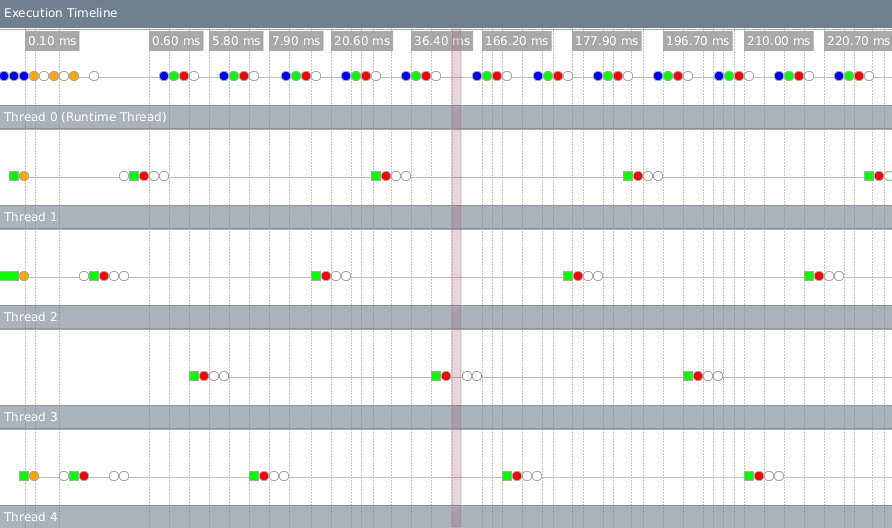
\includegraphics[bb=0 0 892 528, scale=0.4]{images/futures_visualizer_untyped.png}
  \end{center}
  \caption{Screenshot from the Future Visualizer showing the execution timeline
    for the untyped Michael-Scott Queue implementation.}
  \label{fig:untyped-visualizer}
\end{figure}

According to Swaine et al. \cite{swaine_seeing_2012}, programms written in Typed
Racket have advantages over programms written in plain Racket, when it comes to
parallelism. When a parallel program is compiled, the Racket compiler determines
the safety of the code for parallel execution. If the program does not fulfill
all requirements, a so called ``slow path'' will be triggered\footnote{See
  \url{} for details.}, leading
eventually towards sequential execution with the additional overhead paid for
managing parallel processes on top.

Swaine et al. claim that typing the program in Typed Racket counters this
behavior, as they also demonstrate in \cite{swaine_seeing_2012}. It makes
therefore sense to measure the amount of parallel work and compare the typed and
the untyped implementation of the Michael-Scott Queue.

Fig. \ref{fig:untyped-visualizer} shows how the untyped implementation does not
perform work in parallel at all. Instead, each thread pauses entirely as soon as
another thread touches the queue.

\begin{figure}[t]
  \begin{center}
   % \includegraphics[bb=0 0 892 528, scale=0.4]{images/futures_visualizer_typed.png}
  \end{center}
  \caption{Screenshot from the Future Visualizer showing the execution timeline
    for the typed Michael-Scott Queue implementation.}
  \label{fig:typed-visualizer}
\end{figure}

\section{Conclusion and Future Work}

\bibliographystyle{plain}
\bibliography{SPLG.bib}

\end{document}



